% Chapter 1, version 7 (01V7.tex): 21 September 2026.
% Supersedes the supplied 01V6.tex; existing section/objective labels retained.
% V7: bold problem statement, explained/repositioned risk figure, agreed RQ scope.
% Uses the citation keys already present in the supplied Chapter 1.
% Risk diagram: Images/CH01_02_revised.pdf, with Images/CH01_02.png as fallback.
% The risk diagram is fixed after the Section 1.2 explanation (requires float).
% Optional new figure: Images/CH01_DCEC_DCEW.pdf (prompt supplied separately).
% Threshold values and unfinished experiments are deliberately not asserted.

\chapter{Introduction}

\label{ch:introduction}

\section{From physical to image-based verification}
\label{sec:intro-document-as-image}

Modern identity documents have a long history, including medieval safe-conducts protected by the English Safe Conducts Act 1414 \citep{McHugh2021,SafeConducts1414}. Their value as evidence nevertheless depends on establishing that the document is genuine and belongs to the person presenting it.

The digital-first economy has changed how these documents are checked. Consumers now open bank accounts remotely, and the physical ID may be flattened into a smartphone photograph and examined through software. Remote services can inspect visible security features or incorporate chip reading, but a single photograph cannot provide the same evidence as handling a document or accessing its electronically stored information \parencite{GovUK2018}. NIST's guidelines recognise remote unattended proofing, where automated checks do not require interaction with a proofing agent \citep{nist2025sp80063a}.

This workflow creates different opportunities for cyber criminals. Where an attacker can submit or inject a modified image, the forgery can target the captured pixels without requiring a convincing physical counterfeit. International security and law-enforcement agencies recognise identity and document fraud as facilitating wider criminal activity \parencite{EuropolSOCTA2025, frontex2025ara}. Driven by this changing threat landscape, researchers therefore evaluate both manipulation detection and spatial localisation \citep{LuoICDAR2023,GuanOpenMFC2022} through shared datasets and benchmark competitions organised by bodies such as IAPR and NIST. The first asks whether a document was altered; the second asks where.

Spatial outputs also appear in commercial services. IDVerse reports using a neural network for document authentication, while Shufti provides heatmaps highlighting suspected alterations \citep{LexisNexis2025IDVerse,Shufti2025Heatmaps}. Such maps can support inspection, but neither commercial adoption nor greater spatial detail establishes their correctness.


\section{From performance to dependable evidence}
\label{sec:intro-performance-to-evidence}

\begin{samepage}
\hrule
\vspace{0.6em}
\noindent\textbf{\underline{Problem addressed:}} A correct forgery decision does not establish that the accompanying spatial map identifies the altered region. This thesis investigates whether bounded adversarial perturbations can degrade initially acceptable spatial evidence while preserving that correct decision.\par
 \vspace{0.9em}
\hrule
\end{samepage}
\vspace{0.8em}
Neural forensic detectors learn patterns in image acquisition, editing and compression \parencite{verdoliva2020overview}. TruFor, for example, combines noise-sensitive features with RGB information to produce a spatial anomaly map and a document-level score \parencite{guillaro2023trufor}. These outputs answer different questions and require separate evaluation.

Learned detectors may also exploit dataset-specific shortcuts. Compression or capture-device differences can separate training classes without representing the manipulation itself \parencite{geirhos2020shortcut,Lapuschkin2019CleverHans}. Processing inconsistencies can provide useful forensic evidence, but they may also reflect how the dataset was assembled. The clean-data audit examines this distinction before adversarial degradation is interpreted.

Adversarial perturbations are deliberately optimised pixel modifications that target model behaviour within a specified budget \parencite{goodfellow2015explaining,szegedy2014intriguing}. It is important to consider that a document may already contain a swapped portrait or altered text before a subsequent perturbation is applied. Throughout this study, \emph{clean} means before this additional perturbation; a clean image can therefore already contain a forgery. The concern is that a reviewer receives the correct warning with forgery detection but a less useful indication of where the alteration lies from spatial maps.

Figure~\ref{fig:risk-summary-critical} follows these routes from the document to the detector's outputs. The left-hand branch shows how dataset shortcuts can undermine decisions or spatial evidence before an attack. The right-hand branch separates attacks, that change the decision from those that degrade spatial evidence while preserving it. The highlighted route with double red boxes is the focus of this thesis. The other routes explain the need for clean-data checks and classification-attack controls.

% Fixed here so the diagram follows its explanation and precedes Section 1.3.
\begin{figure}[H]
\centering
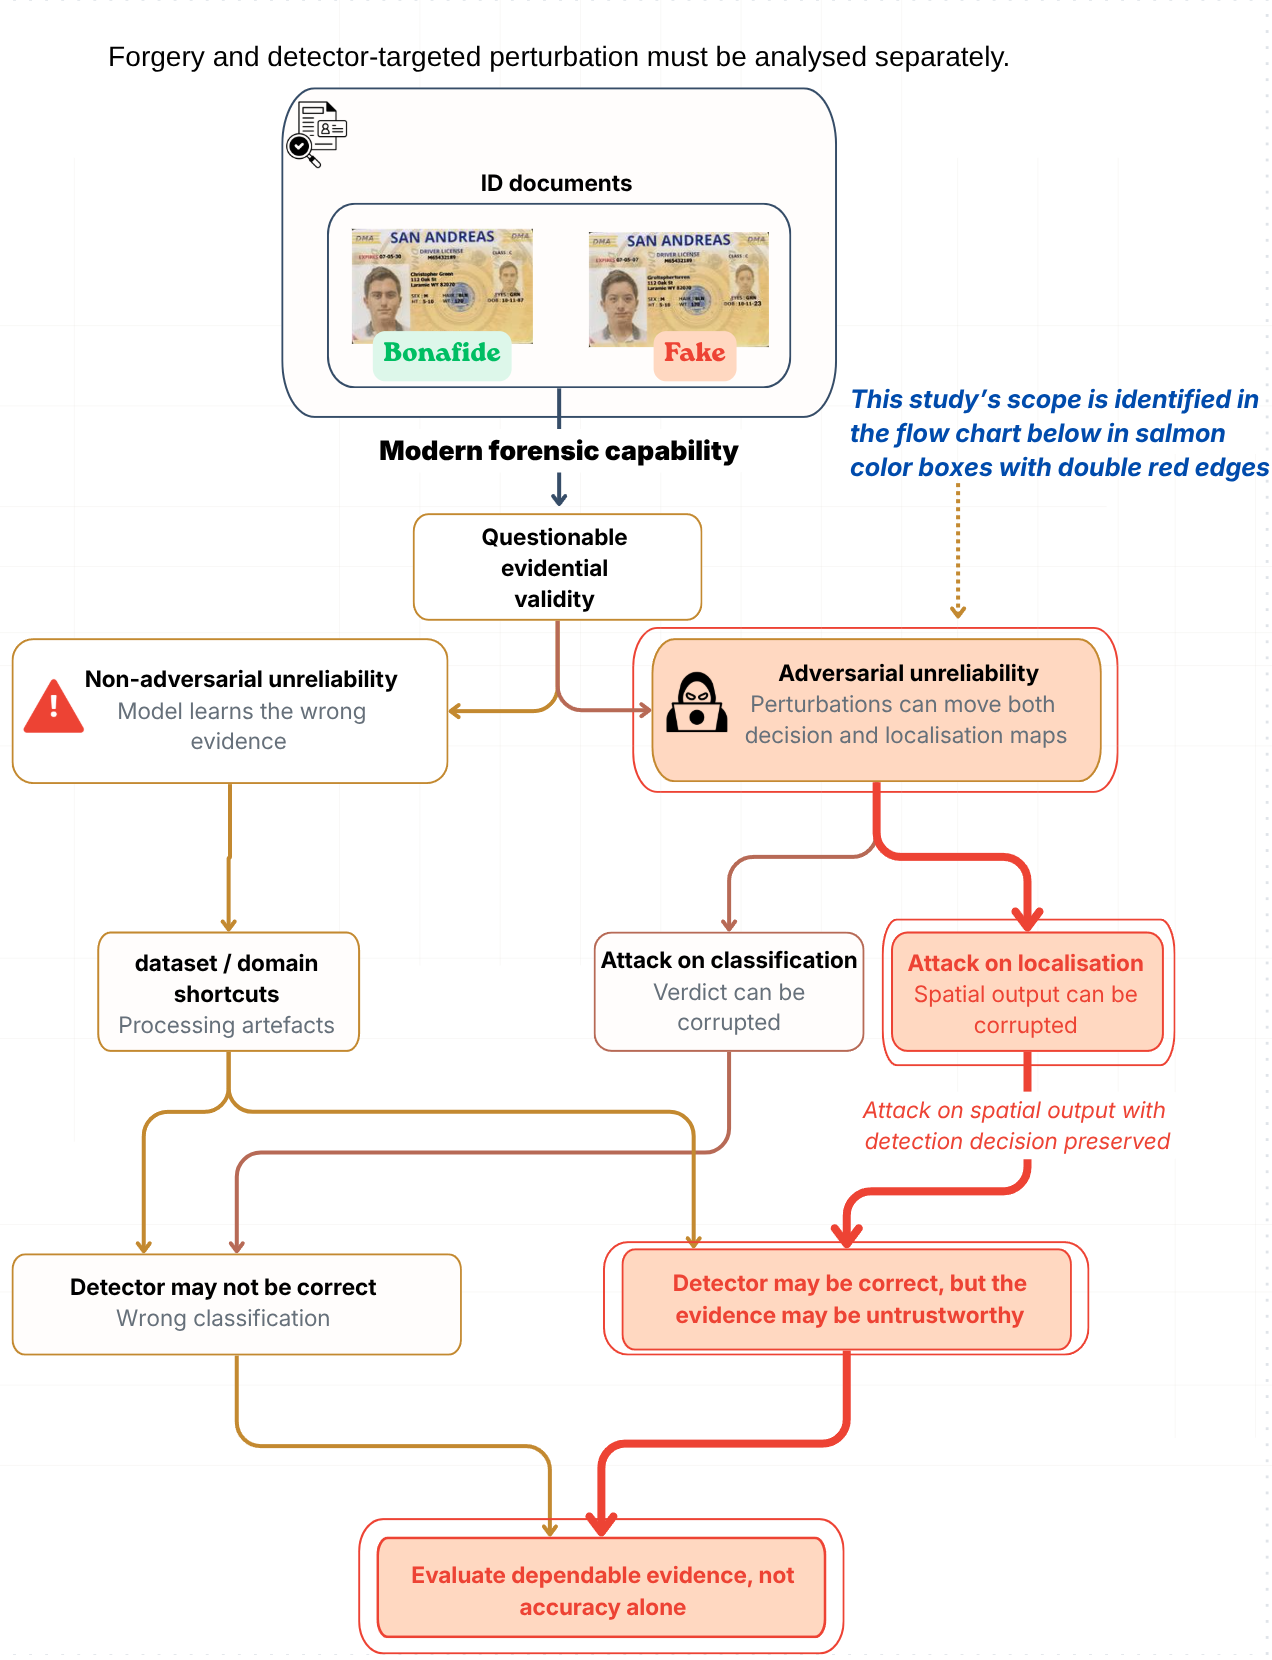
\includegraphics[width=0.95\textwidth,height=0.73\textheight,keepaspectratio]{Images/CH01_02.png}
\caption{Conceptual routes to unreliable forensic outputs. Arrows show possible routes to failure; the highlighted route with double red boxes concerns degradation of spatial evidence while the correct forgery decision is preserved.}
\label{fig:risk-summary-critical}
\end{figure}
%------------------------------------------------------------------
\clearpage
\section{Two ways of producing spatial evidence, and what is not known}
\label{sec:intro-two-paradigms-gap}

Learned detectors produce spatial evidence in two different ways.

\begin{enumerate}
    \item \textbf{Post-hoc attribution:} A classifier returns a score, and an attribution method such as Grad-CAM is applied afterwards to indicate regions contributing to the target score \parencite{Selvaraju2017GradCAM}. The map is an inference about the classifier, rather than an output it was trained to produce.
    \item \textbf{Native manipulation-localisation:} A purpose-built system such as TruFor is trained to estimate manipulated regions directly. Its spatial map is a supervised prediction, accompanied by confidence and detection outputs \parencite{guillaro2023trufor}.
\end{enumerate}

These outputs have different meanings. Agreement with manipulation annotations asks whether a map identifies the labelled regions. Explanation faithfulness asks whether it reflects the classifier's behaviour. This study concerns the first property and its vulnerability to attack; spatial agreement alone does not establish the second.

Earlier work demonstrates prediction-preserving attacks on explanations and attacks on forensic localisers \parencite{ghorbani2019fragile,dombrowski2019explanations,cao2024transferable}. The studies reviewed in Chapter~2 do not establish how initially acceptable spatial evidence degrades under a decision-preserving constraint in both kinds of pipeline on identity-document images.

FantasyID supplies complete document images, physical print-and-capture conditions, manipulated face and text regions, and public annotations \parencite{korshunov2025fantasyid}. ResNet-18 with Grad-CAM and TruFor represent the two routes. Each pipeline is evaluated against its own clean performance. The aim is to measure vulnerability within that performance, rather than to develop a higher-scoring detector.

The analysis follows three stages:
\begin{enumerate}
    \item \textbf{DC(Decision Correct):} Identify manipulated images correctly classified before adversarial perturbation.
    \item \textbf{DCEC(Decision Correct, Evidence Correct):} Within DC, retain images whose clean maps meet both a relevance-mass requirement and a relevance-rank-overlap requirement against the annotations.
    \item \textbf{DCEW(Decision Correct, Evidence Wrong):} Within the fixed clean DCEC set, count attacks that preserve the correct decision but cause either evidence requirement to fail.
\end{enumerate}

Relevance mass accuracy ($E$) measures how much map mass lies inside the annotation. Relevance rank accuracy (RRA) measures how far a set of the strongest map pixels, equal in size to the annotated region, overlaps it. ``Evidence correct'' therefore means passing this study's spatial criterion. The protocol requires thresholds to be calibrated using clean development evidence and fixed before evaluating DCEC-to-DCEW outcomes. Both pipelines follow the same calibration procedure, although their numerical thresholds may differ. Within each pipeline, the same thresholds apply to clean and adversarial maps.

Reporting the numbers reaching DC and DCEC keeps limited coverage visible. Classification flips remain in the DCEC denominator and are reported separately. Images qualifying for both pipelines provide an additional view of each pipeline's degradation; they do not remove differences in architecture, training or map resolution.

% This figure is included automatically once the prompted artwork is added.
\IfFileExists{Images/CH01_DCEC_DCEW.pdf}{%
Figure~\ref{fig:dc-dcec-dcew} summarises the analysis populations and outcomes.
\begin{figure}[tbp]
\centering
\includegraphics[width=\textwidth,height=0.66\textheight,keepaspectratio]{Images/CH01_DCEC_DCEW.pdf}
\caption{DC, DCEC and adversarial outcomes. Clean eligibility fixes the denominator. An evidence failure counts as DCEW only while the decision remains correct.}
\label{fig:dc-dcec-dcew}
\end{figure}
}{}

\section{Aim, research question and objectives}
\label{sec:intro-aim-rq-objectives}

This dissertation evaluates whether bounded adversarial perturbations can undermine initially acceptable spatial evidence while preserving a correct identity-document forgery decision.

\begin{quote}
\noindent\textbf{Research question.} To what extent can bounded adversarial perturbations degrade initially acceptable spatial evidence from post-hoc attribution and native localisation while preserving the correct identity-document forgery decision?
\end{quote}

This question is investigated using ResNet-18 with Grad-CAM and TruFor. Each pipeline is evaluated against its own clean performance. Chapter~2 explains the reasons for selecting these models.

The following five objectives address this question.

\crefname{enumi}{objective}{objectives}
\Crefname{enumi}{Objective}{Objectives}
\begingroup
\renewcommand{\theenumi}{O\arabic{enumi}}
\renewcommand{\labelenumi}{\textbf{\theenumi.}}
\begin{enumerate}
    \item\label{obj:baselines} Establish clean detection and spatial-agreement baselines under documented preprocessing, reporting the images and forgery families each pipeline can support.
    \item\label{obj:evidence} Audit compression-related cues and regional sensitivity, and calibrate the joint $E$ and RRA criterion using clean-development measurements and a visual review conducted without access to those measurements.
    \item\label{obj:attack} Evaluate bounded, white-box attacks on spatial evidence, measuring DCEC-to-DCEW transitions and continuous degradation while reporting decision preservation. Use classification-targeted attacks as complementary controls.
    \item\label{obj:compare} Assess each pipeline against its own clean baseline, quantify uncertainty using document-stem resampling, and examine shared eligible images and visual examples as an additional analytical view.
    \item\label{obj:implications} Synthesise the findings to identify when spatial outputs support manipulation assessment, explaining the practical value, remaining risks and limits of the evidence.
\end{enumerate}
\endgroup

\section{Contribution}
\label{sec:intro-contribution}

The contribution is an evaluation of attacks that undermine spatial evidence while preserving correct forgery decisions. Its outputs are clean coverage estimates, conditional DCEC-to-DCEW rates and continuous changes in spatial agreement. The clean audit supplies the context needed to distinguish an attack-induced failure from evidence that was already inadequate.

For financial-services practitioners, the study examines whether a map accompanying a correct forgery warning can become less useful for inspecting the document. It does not demonstrate a verification bypass or measure how human reviewers respond. For researchers, it provides a documented evaluation framework and experimental evidence for studying this failure.

The claims remain bounded by the selected dataset, pipelines and attack configurations. Rectangular annotations approximate manipulated regions, and the maps differ in meaning and resolution. These limits remain relevant when interpreting degradation relative to each pipeline's clean baseline.

\section{Structure of the dissertation}
\label{sec:intro-structure}

Chapter~2 reviews the datasets, spatial outputs, evaluation measures and adversarial literature. Chapter~3 defines the methodology, calibration and risk controls. Chapter~4 reports clean performance and DCEC coverage; Chapter~5 evaluates adversarial degradation. Chapter~6 discusses the findings and concludes. Supporting detail is organised in Appendix~A for metric calibration and sensitivity checks, Appendices~B and~C for ResNet-18 and TruFor decisions and risk registers, and Appendix~D for reproducibility records.
